In this section we would like to show how we can apply universal autotuning 
and collaboratively found optimization solutions to several popular workloads
used by RPi community: \textit{zlib decode, zlib encode, 
7z encode, aubio, ccrypt, gzip decode, gzip encode, minigzip decode, 
minigzip encode, rhash, sha512sum, unrar}.
%
We added the latest versions of these real programs 
to the CK describing how to compile and run them 
using CK JSON meta data:

\begin{flushleft}
\texttt{\$ ck ls ck-rpi-optimization:program:*}
\end{flushleft}

We can now autotune any of these programs via CK as described in Section~\ref{sec:flag_autotuning}.
%
For example, the following command will autotune \textit{zlib decode} workload
with 150 random combinations of compiler flags including parametric and architecture 
specific ones, and will record results in a local repository:

\begin{flushleft}
\texttt{\$ ck autotune program:zlib --cmd\_key=decode
  --iterations=150 --repetitions=3 
  --scenario=experiment.tune.compiler.flags.gcc
  --parametric\_flags --cpu\_flags --base\_flags 
  --record\_uoa=tmp-rpi3-zlib-decode-gcc4-150bpc-rnd}
\end{flushleft}

Figure~\ref{fig:autotuning-zlib-decode-gcc4} 
(\href{http://cknowledge.org/repo/web.php?wcid=graph:3a97d1f6494f9d45&subgraph=rpi3-autotuning-zlib-decode-gcc4-interactive}{link with interactive graph}) 
shows manually annotated graph with the outcome of such autotuning 
when using GCC 4.9.2 compiler on RPi3 device
in terms of execution time with variation and code size.
%
Each blue point on this graph is related to one combination of random compiler flags.
%
Red line highlights the frontier of all autotuning results 
to let users trade off execution time and code size 
during multi-objective optimization.
%
Similar to graphs in Section~\ref{sec:flag_autotuning}, we also plotted points 
when using several main GCC and Clang optimization levels.

   % === zlib decode GCC 4.9.2 ==================================================================
   %CK={"action":"prepare_for_latex", "cid":"slide:b6184e4db89cddce", "file":"22f5af13e8e498aa-cropped.pdf", "path":"ck-assets", "ck_image":"yes", "ck_image_width":900}
   %CK={"action":"prepare_for_latex", "cid":"slide:b6184e4db89cddce", "file":"22f5af13e8e498aa-table1.tex", "uid":"ea356adf24643d69", "path":"ck-assets"}
   %CK={"action":"prepare_for_latex", "cid":"slide:b6184e4db89cddce", "file":"22f5af13e8e498aa-table1.html", "uid":"ea356adf24643d69", "path":"ck-assets"}
   \begin{figure*}[!htbp]
     \centering
      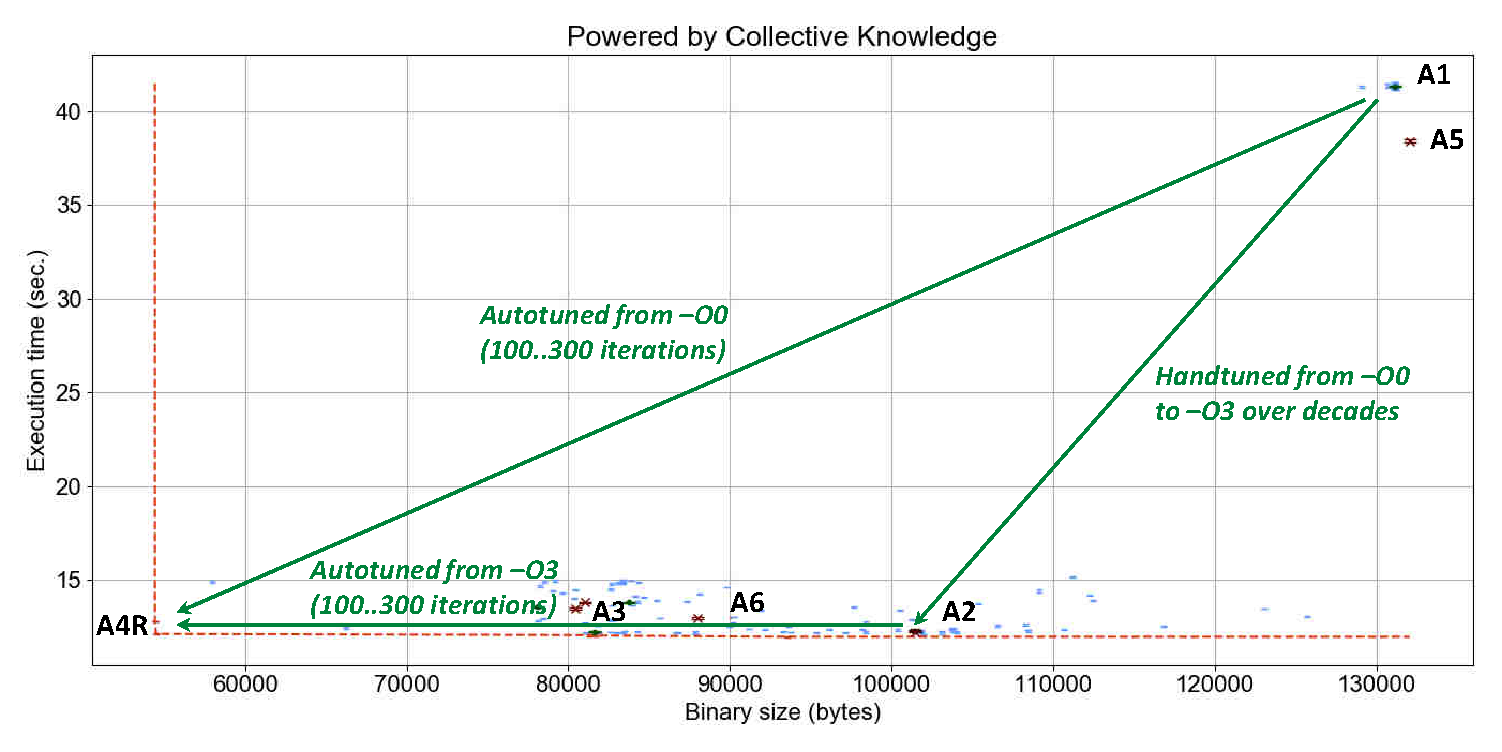
\includegraphics[width=5.2in]
      {ck-assets/22f5af13e8e498aa-cropped.pdf} %CK_URL={22f5af13e8e498aa-cropped.pdf}
      \vspace{0.1in}
          \begin{tabular}{|l|l|l|l|p{3.2in}|}
     \hline
      \textbf{ID} & \textbf{Compiler} & \textbf{Time (sec.)} & \textbf{Size (bytes)} & \textbf{Flags} \\ 
     \hline
      \textbf{ A1 } &  GCC 4.9.2  &  41.3 $\pm$ 0.0  &  131140  & {\small  }\\
     \hline
      \textbf{ A2 } &  GCC 4.9.2  &  12.2 $\pm$ 0.0  &  101448  & {\small -O3 }\\
     \hline
      \textbf{ A3 } &  GCC 4.9.2  &  13.6 $\pm$ 0.0  &  78116  & {\small -Os }\\
     \hline
      \textbf{ A4R } &  GCC 4.9.2  &  12.1 $\pm$ 0.1  &  54272  & {\small -O2 -flto -fno-tree-fre }\\
     \hline
      \textbf{ A5 } &  CLANG 3.8.1  &  38.5 $\pm$ 0.0  &  132080  & {\small  }\\
     \hline
      \textbf{ A6 } &  CLANG 3.8.1  &  12.9 $\pm$ 0.1  &  90076  & {\small -O3 }\\
     \hline
    \end{tabular}     %CK_HTML={ck-assets/22f5af13e8e498aa-table1.html}
      \vspace{0.1in}
     \caption{
      Results of GCC 4.9.2 random compiler flag autotuning of a zlib decode workload on RPi3
      device using CK with a highlighted frontier (trading-off execution time and code size) 
      and best found combinations of flags on this frontier.
     }
     \label{fig:autotuning-zlib-decode-gcc4}
   \end{figure*}

In contrast with \textit{susan corners} workload, autotuning did not improve execution time 
of \textit{zlib decode} over \textit{-O3} level most likely because this algorithm is present
in many benchmarking suits. 
%
On the other hand, autotuning impressively improved code size over \textit{-O3} 
by nearly 2x without sacrificing execution time, and by ~1.5x with 11\% execution time
improvement over \textit{-Os} (reduced optimization solution \textbf{A4R}), 
showing that code size optimization is still a second class citizen.

Since local autotuning can still be quite costly (150 iterations to achieve above results),
we can now first check 10..20 most efficient combinations of compiler flags 
already found and shared by the community for this compiler and hardware
(Figure~\ref{fig:ck-snapshot-of-results-gcc4}).
%
Note that programs from this section did not participate in crowd-tuning
to let us have a fair evaluation of the influence of shared optimizations 
on these programs similar to leave-one-out cross-validation in machine learning.

Figure~\ref{fig:autotuning-zlib-decode-gcc4-reactions} shows "reactions" 
of \textit{zlib decode} to these optimizations in terms of execution time and code size 
(\href{http://cknowledge.org/repo/web.php?wcid=graph:47f0b282396776c4&subgraph=rpi3-autotuning-zlib-decode-gcc4-reactions-interactive}{online interactive graph}).
%
We can see that crowd-tuning solutions indeed cluster in a relatively small area 
close to \textit{-O3} with one collaborative solution (\textbf{C1}) close to the 
best optimization solution found during lengthy autotuning (\textbf{A4R}) 
thus providing a good trade off between autotuning time, execution time and code size.

   % === zlib decode GCC 4.9.2 reactions ==================================================================
   %CK={"action":"prepare_for_latex", "cid":"slide:02c571571ee45d4a", "file":"749a8998a2e29db5-cropped.pdf", "path":"ck-assets", "ck_image":"yes", "ck_image_width":900}
   %CK={"action":"prepare_for_latex", "cid":"slide:02c571571ee45d4a", "file":"749a8998a2e29db5-table1.tex", "uid":"47ae2170c78ef192", "path":"ck-assets"}
   %CK={"action":"prepare_for_latex", "cid":"slide:02c571571ee45d4a", "file":"749a8998a2e29db5-table1.html", "uid":"47ae2170c78ef192", "path":"ck-assets"}
   \begin{figure*}[!htbp]
     \centering
      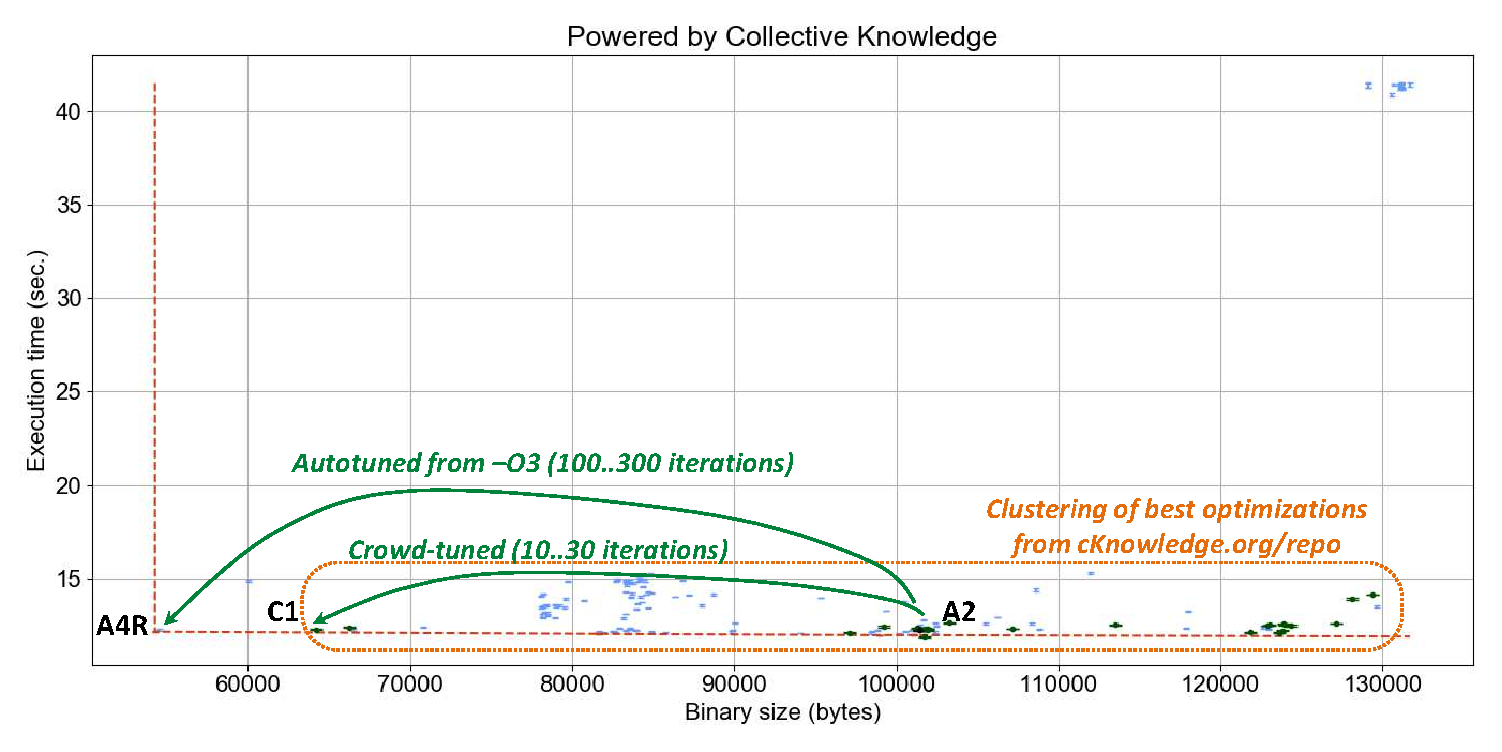
\includegraphics[width=5.2in]
      {ck-assets/749a8998a2e29db5-cropped.pdf} %CK_URL={749a8998a2e29db5-cropped.pdf}
      \vspace{0.1in}
          \begin{tabular}{|l|l|l|l|p{3.2in}|}
     \hline
      \textbf{ID} & \textbf{Compiler} & \textbf{Time (sec.)} & \textbf{Size (bytes)} & \textbf{Flags} \\ 
     \hline
      \textbf{ \href{http://cknowledge.org/repo/web.php?wcid=experiment:9b2b24a80c45aa9b\&subpoint=eb28149e9a71762d}{A2} } &  GCC 4.9.2  &  12.2 $\pm$ 0.0  &  101448  & {\small -O3 }\\
     \hline
      \textbf{ \href{http://cknowledge.org/repo/web.php?wcid=experiment:f5489592a3a15bf3\&subpoint=6236b2e4742629aa}{A4R} } &  GCC 4.9.2  &  12.1 $\pm$ 0.1  &  54272  & {\small -O2 -flto -fno-tree-fre }\\
     \hline
      \textbf{ \href{http://cknowledge.org/repo/web.php?wcid=experiment:dfc49b5be33c1813\&subpoint=ec6a2e99da2e3445}{C1} } &  GCC 4.9.2  &  12.2 $\pm$ 0.1  &  64184  & {\small -O3 -fno-inline -flto }\\
     \hline
    \end{tabular}     %CK_HTML={ck-assets/749a8998a2e29db5-table1.html}
      \vspace{0.1in}
     \caption{
      Speeding up GCC 4.9.2 autotuning of a zlib decode workload on RPi3 device using 
      10..20 best performing combinations of compiler flags already found and shared by the community
      during crowd-tuning.
     }
     \label{fig:autotuning-zlib-decode-gcc4-reactions}
   \end{figure*}
   %\url{http://cknowledge.org/repo/web.php?wcid=graph:47f0b282396776c4&subgraph=rpi3-autotuning-zlib-decode-gcc4-reactions-interactive}

Autotuning \textit{zlib decode} using \textit{GCC 7.1.0} revels even more interesting results
in comparison with \textit{susan corners} as shown in Figure~\ref{fig:autotuning-zlib-decode-gcc7} 
(\href{http://cknowledge.org/repo/web.php?wcid=graph:2bf38fd88a0e3ba1&subgraph=rpi3-autotuning-zlib-decode-gcc7-interactive}{online interactive graph}).
%
While there is practically no execution time improvements when switching from \textit{GCC 4.9.2} to \textit{GCC 7.1.0}
on \textit{-O3} and \textit{-Os} optimization levels, \textit{GCC 7.1.0 -O3} considerably degraded code size by nearly 20\%.
%
Autotuning also shows few opportunities on \textit{GCC 7.1.0} in comparison with \textit{GCC 4.9.2}
where best found optimization \textbf{B4R} is worse in terms of code size than \textbf{A4R} also by around 20\%.
%
These results highlight issues which both end-users and compiler designers face
when searching for efficient combinations of compiler flags or preparing the 
default optimization levels -Ox.

   % === zlib decode GCC 7.1.0 ==================================================================
   %CK={"action":"prepare_for_latex", "cid":"slide:f69ffd7894e87b73", "file":"3f15a01f17d48b7b-cropped.pdf", "path":"ck-assets", "ck_image":"yes", "ck_image_width":900}
   %CK={"action":"prepare_for_latex", "cid":"slide:f69ffd7894e87b73", "file":"3f15a01f17d48b7b-table1.tex", "uid":"3eb68b45a4bda8e9", "path":"ck-assets"}
   %CK={"action":"prepare_for_latex", "cid":"slide:f69ffd7894e87b73", "file":"3f15a01f17d48b7b-table1.html", "uid":"3eb68b45a4bda8e9", "path":"ck-assets"}
   \begin{figure*}[!htbp]
     \centering
      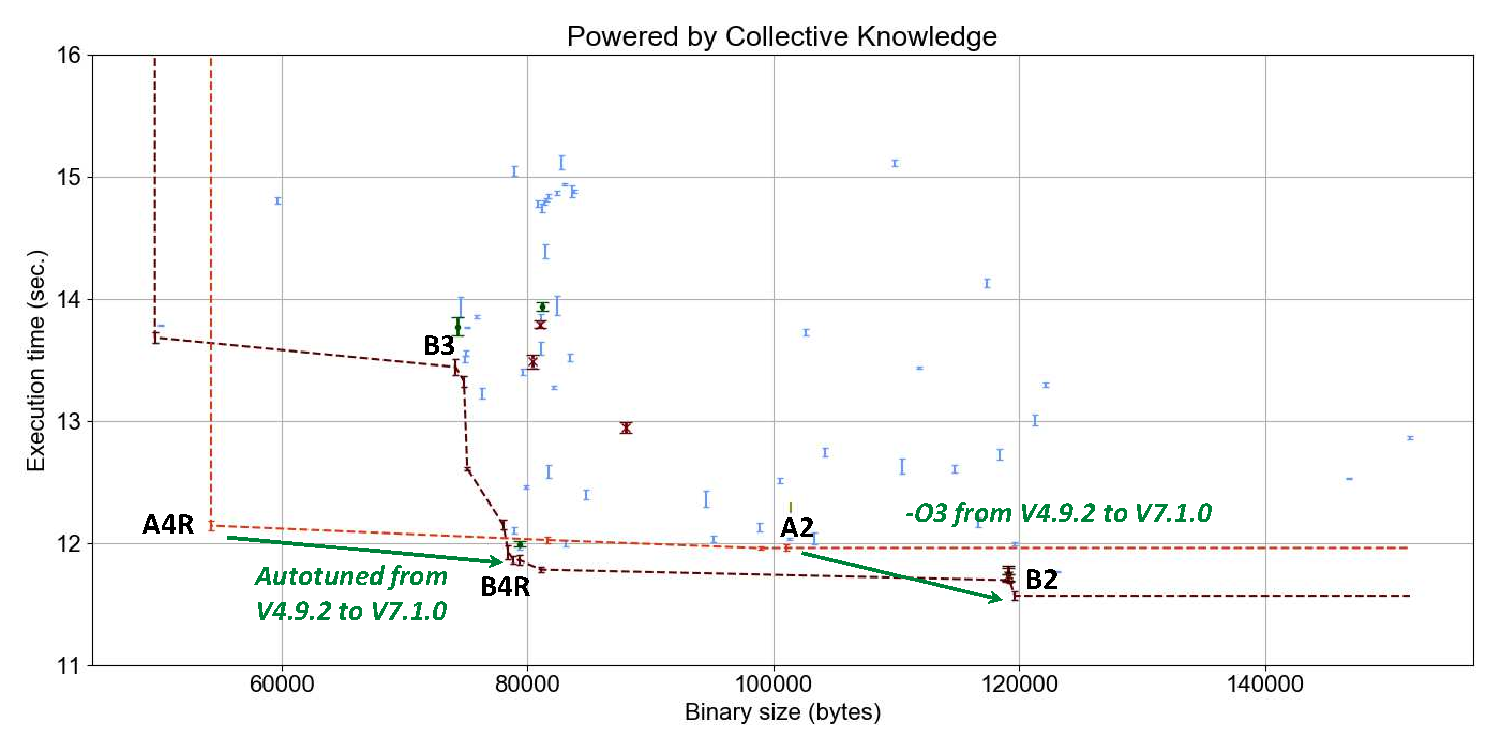
\includegraphics[width=5.2in]
      {ck-assets/3f15a01f17d48b7b-cropped.pdf} %CK_URL={3f15a01f17d48b7b-cropped.pdf}
      \vspace{0.1in}
          \begin{tabular}{|l|l|l|l|p{3.2in}|}
     \hline
      \textbf{ID} & \textbf{Compiler} & \textbf{Time (sec.)} & \textbf{Size (bytes)} & \textbf{Flags} \\ 
     \hline
      \textbf{ A2 } &  GCC 4.9.2  &  12.2 $\pm$ 0.0  &  101448  & {\small -O3 }\\
     \hline
      \textbf{ A4R } &  GCC 4.9.2  &  12.1 $\pm$ 0.1  &  54272  & {\small -O2 -flto -fno-tree-fre }\\
     \hline
      \textbf{ B1 } &  GCC 7.1.0  &  41.3 $\pm$ 0.0  &  128376  & {\small  }\\
     \hline
      \textbf{ B2 } &  GCC 7.1.0  &  11.7 $\pm$ 0.1  &  119084  & {\small -O3 }\\
     \hline
      \textbf{ B3 } &  GCC 7.1.0  &  13.7 $\pm$ 0.1  &  74280  & {\small -Os }\\
     \hline
      \textbf{ B4R } &  GCC 7.1.0  &  11.9 $\pm$ 0.1  &  78700  & {\small -O2 -fno-early-inlining -fno-tree-fre }\\
     \hline
    \end{tabular}     %CK_HTML={ck-assets/3f15a01f17d48b7b-table1.html}
      \vspace{0.1in}
     %CK_INTERACTIVE_GRAPH_PASSIVE={"cid":"2d41f89bcf32d4d4:2bf38fd88a0e3ba1", "where":"div#ck_interactive_a30267d0c344fcdb", "html":"rpi3-autotuning-zlib-decode-gcc7-interactive.html", "style":"rpi3-autotuning-zlib-decode-gcc7-interactive.style", "add_div":"yes", "add_box":"yes", "box_width":700, "remove_script_src":"yes"}
     \caption{
       Results of GCC 7.1.0 random compiler flag autotuning of zlib decode on RPi3 device 
       with a highlighted frontier (trading-off execution time and code size), 
       best combinations of flags on this frontier, and comparison with the results from GCC 4.9.2.
     }
     \label{fig:autotuning-zlib-decode-gcc7}
   \end{figure*}
   %\url{http://cknowledge.org/repo/web.php?wcid=graph:2bf38fd88a0e3ba1&subgraph=rpi3-autotuning-zlib-decode-gcc7-interactive}

CK crowd-tuning can assist in this case too - Figure~\ref{fig:autotuning-zlib-decode-gcc7-reactions}
shows reactions of \textit{zlib decode} to the most efficient combinations of GCC 7.1.0 compiler flags
shared by the community for RPi3 
(\href{http://cknowledge.org/repo/web.php?wcid=graph:a53089441c68c978&subgraph=rpi3-autotuning-zlib-decode-gcc7-reactions-interactive}{online interactive graph}).
%
Shared optimization solution~\textbf{C2} achieved the same results in terms of execution time and code size
as reduced solution \textbf{B4R} found during 150 random autotuning iterations.
%
Furthermore, another shared optimization solution~\textbf{C1} improved code size by ~15\% in comparison
with GCC 7.1.0 autotuning solution~\textbf{B4R} and is close to the best solution GCC 4.9.2 autotuning solution~\textbf{A4R}.
%
These results suggest that 150 iterations with random combinations of compiler flags 
may not be enough to find efficient solution for \textit{zlib decode}.
%
In turn, crowd-tuning can help considerably accelerate and focus such optimization space exploration.

   % === zlib decode GCC 7.1.0 reactions ==================================================================
   %CK={"action":"prepare_for_latex", "cid":"slide:a75a7d4898bcfb24", "file":"74ba8b07475626f5-cropped.pdf", "path":"ck-assets", "ck_image":"yes", "ck_image_width":900}
   %CK={"action":"prepare_for_latex", "cid":"slide:a75a7d4898bcfb24", "file":"74ba8b07475626f5-table1.tex", "uid":"f3925ee82fa445da", "path":"ck-assets"}
   %CK={"action":"prepare_for_latex", "cid":"slide:a75a7d4898bcfb24", "file":"74ba8b07475626f5-table1.html", "uid":"f3925ee82fa445da", "path":"ck-assets"}
   \begin{figure*}[!htbp]
     \centering
      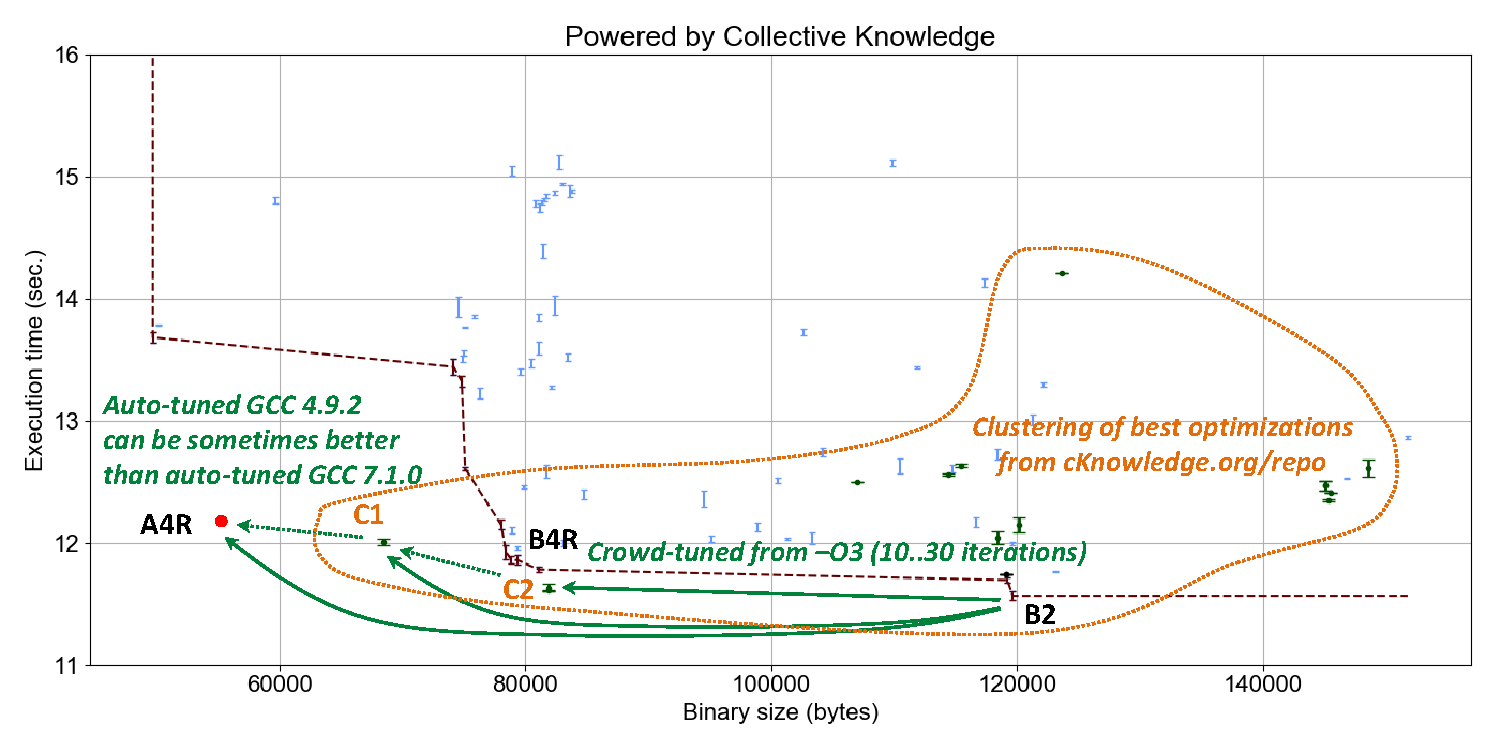
\includegraphics[width=5.2in]
      {ck-assets/74ba8b07475626f5-cropped.pdf} %CK_URL={74ba8b07475626f5-cropped.pdf}
      \vspace{0.1in}
          \begin{tabular}{|l|l|l|l|p{3.2in}|}
     \hline
      \textbf{ID} & \textbf{Compiler} & \textbf{Time (sec.)} & \textbf{Size (bytes)} & \textbf{Flags} \\ 
     \hline
      \textbf{ A4R } &  GCC 4.9.2  &  12.1 $\pm$ 0.1  &  54272  & {\small -O2 -flto -fno-tree-fre }\\
     \hline
      \textbf{ B2 } &  GCC 7.1.0  &  11.7 $\pm$ 0.1  &  119084  & {\small -O3 }\\
     \hline
      \textbf{ B4R } &  GCC 7.1.0  &  11.9 $\pm$ 0.1  &  78700  & {\small -O2 -fno-early-inlining -fno-tree-fre }\\
     \hline
      \textbf{ C1 } &  GCC 7.1.0  &  12.0 $\pm$ 0.0  &  68464  & {\small -O3 -fno-inline -flto }\\
     \hline
      \textbf{ C2 } &  GCC 7.1.0  &  11.6 $\pm$ 0.1  &  81880  & {\small -O3 -flto }\\
     \hline
    \end{tabular}     %CK_HTML={ck-assets/74ba8b07475626f5-table1.html}
      \vspace{0.1in}
     \caption{
      Testing reactions of zlib decode to top most efficient GCC 7.1.0 optimizations shared by the community for RPi3 devices vs GCC 4.9.2.
     }
     \label{fig:autotuning-zlib-decode-gcc7-reactions}
   \end{figure*}
   %\url{http://cknowledge.org/repo/web.php?wcid=graph:a53089441c68c978&subgraph=rpi3-autotuning-zlib-decode-gcc7-reactions-interactive}

We performed the same autotuning and crowd-tuning experiments for \textit{zlib encode} workload
with results shown in Figures~\ref{fig:autotuning-zlib-encode-gcc4},~\ref{fig:autotuning-zlib-encode-gcc4-reactions},~\ref{fig:autotuning-zlib-encode-gcc7},~\ref{fig:autotuning-zlib-encode-gcc7-reactions}.
%
The results show similar trend that \textit{-O3} optimization level of both \textit{GCC 4.7.2} and \textit{GCC 7.1.0} 
perform well in terms of execution time, while there is the same degradation in code size when moving to a new compiler
(since we monitor the whole zlib binary size for both decode and encode functions).
%
Crowd-tuning also helped improve code size though optimizations~\textbf{A4R},~\textbf{B4R} and \textbf{C1}
are not the same as in case of \textit{zlib decode}.
%
The reason is that algorithms are different and need different optimizations 
to keep execution time intact while improving code size.
%
Such result provides an extra motivation for function-level optimizations
already available in GCC.

   % === zlib encode GCC 4.9.2 ==================================================================
   %CK={"action":"prepare_for_latex", "cid":"slide:d8a2cc151f814d9b", "file":"269da4a48ecdfe46-cropped.pdf", "path":"ck-assets", "ck_image":"yes", "ck_image_width":900}
   %CK={"action":"prepare_for_latex", "cid":"slide:d8a2cc151f814d9b", "file":"269da4a48ecdfe46-table1.tex", "uid":"d79932c49ea93b8b", "path":"ck-assets"}
   %CK={"action":"prepare_for_latex", "cid":"slide:d8a2cc151f814d9b", "file":"269da4a48ecdfe46-table1.html", "uid":"d79932c49ea93b8b", "path":"ck-assets"}
   \begin{figure*}[!htbp]
     \centering
      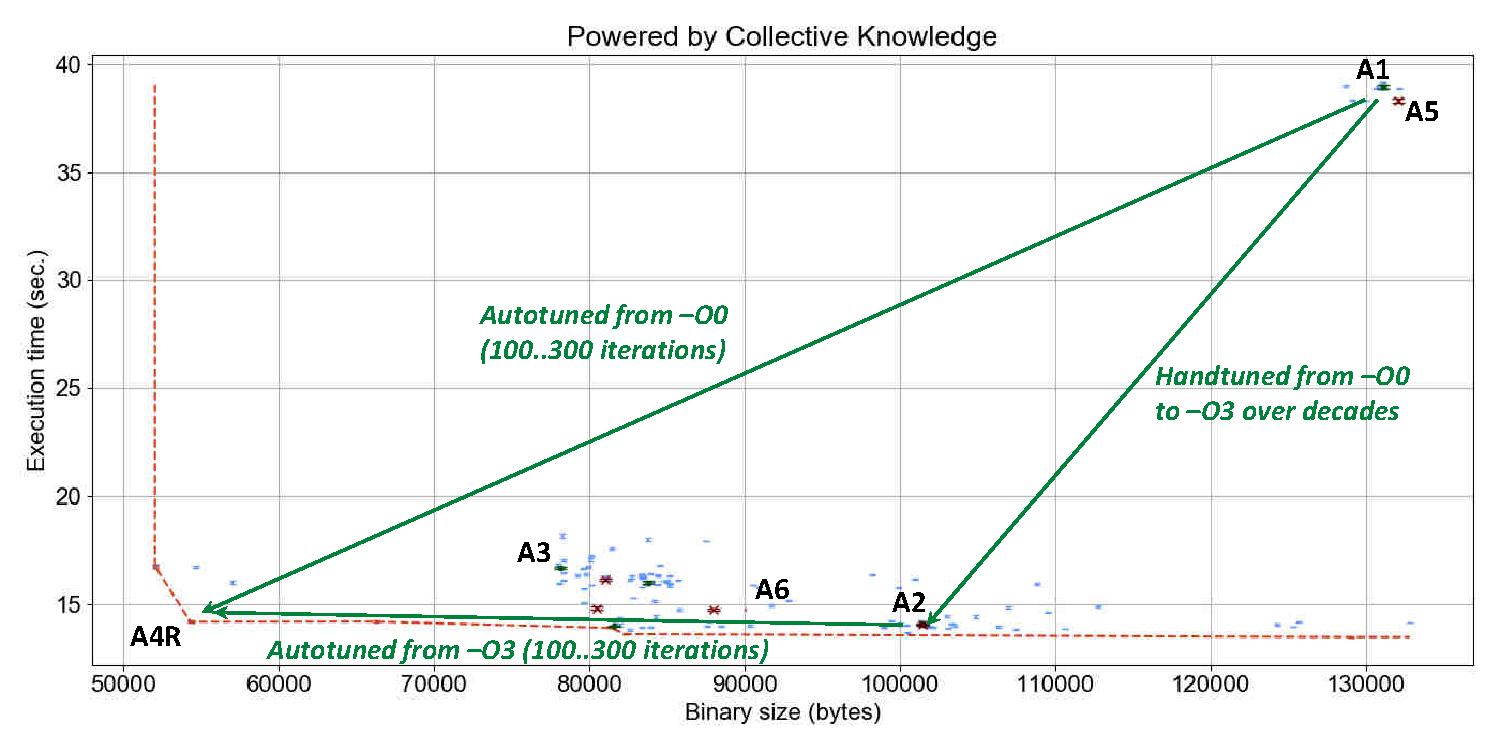
\includegraphics[width=5.2in]
      {ck-assets/269da4a48ecdfe46-cropped.pdf} %CK_URL={269da4a48ecdfe46-cropped.pdf}
      \vspace{0.1in}
          \begin{tabular}{|l|l|l|l|p{3.2in}|}
     \hline
      \textbf{ID} & \textbf{Compiler} & \textbf{Time (sec.)} & \textbf{Size (bytes)} & \textbf{Flags} \\ 
     \hline
      \textbf{ A1 } &  GCC 4.9.2  &  39.0 $\pm$ 0.1  &  131140  & {\small  }\\
     \hline
      \textbf{ A2 } &  GCC 4.9.2  &  14.0 $\pm$ 0.1  &  101448  & {\small -O3 }\\
     \hline
      \textbf{ A3 } &  GCC 4.9.2  &  16.7 $\pm$ 0.1  &  78116  & {\small -Os }\\
     \hline
      \textbf{ A4R } &  GCC 4.9.2  &  14.2 $\pm$ 0.1  &  54284  & {\small -O2 -flto }\\
     \hline
      \textbf{ A5 } &  CLANG 3.8.1  &  38.2 $\pm$ 0.1  &  132080  & {\small  }\\
     \hline
      \textbf{ A6 } &  CLANG 3.8.1  &  14.7 $\pm$ 0.1  &  90076  & {\small -O3 }\\
     \hline
    \end{tabular}     %CK_HTML={ck-assets/269da4a48ecdfe46-table1.html}
      \vspace{0.1in}
     \caption{
      Results of GCC 4.9.2 random compiler flag autotuning of a zlib encode workload on RPi3
      device using CK with a highlighted frontier (trading-off execution time and code size) 
      and best found combinations of flags on this frontier.
     }
     \label{fig:autotuning-zlib-encode-gcc4}
   \end{figure*}

   %\url{http://cknowledge.org/repo/web.php?wcid=graph:3e5db47f4a15bad9&subgraph=rpi3-autotuning-zlib-encode-gcc4-interactive}


   % === zlib encode GCC 4.9.2 reactions ==================================================================
   %CK={"action":"prepare_for_latex", "cid":"slide:b861d0e44e2ae283", "file":"8d7b4b7a7b8545e7-cropped.pdf", "path":"ck-assets", "ck_image":"yes", "ck_image_width":900}
   %CK={"action":"prepare_for_latex", "cid":"slide:b861d0e44e2ae283", "file":"8d7b4b7a7b8545e7-table1.tex", "uid":"843bd97e47a6bd5b", "path":"ck-assets"}
   %CK={"action":"prepare_for_latex", "cid":"slide:b861d0e44e2ae283", "file":"8d7b4b7a7b8545e7-table1.html", "uid":"843bd97e47a6bd5b", "path":"ck-assets"}
   \begin{figure*}[!htbp]
     \centering
      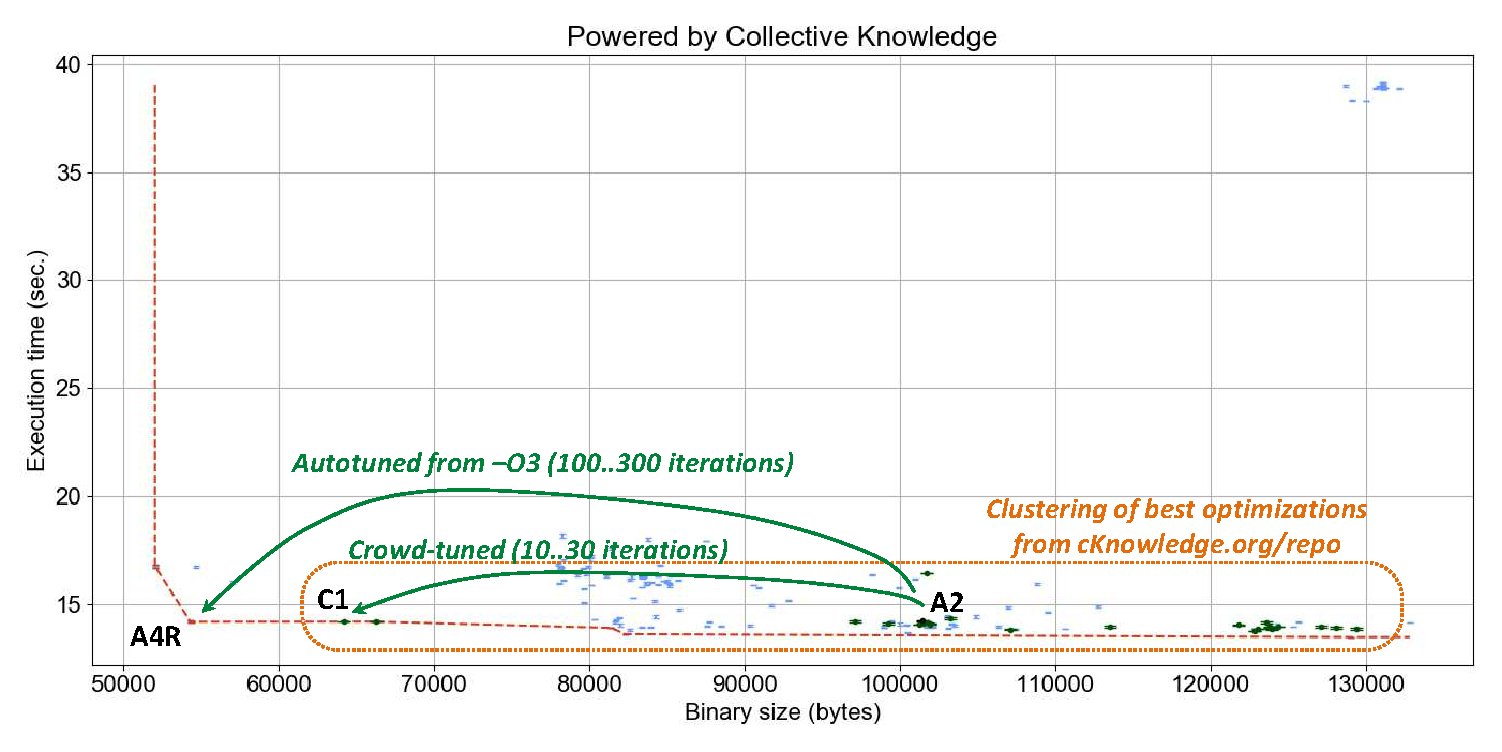
\includegraphics[width=5.8in]
      {ck-assets/8d7b4b7a7b8545e7-cropped.pdf} %CK_URL={8d7b4b7a7b8545e7-cropped.pdf}
      \vspace{0.1in}
          \begin{tabular}{|l|l|l|l|p{3.2in}|}
     \hline
      \textbf{ID} & \textbf{Compiler} & \textbf{Time (sec.)} & \textbf{Size (bytes)} & \textbf{Flags} \\ 
     \hline
      \textbf{ \href{http://cknowledge.org/repo/web.php?wcid=experiment:21f631290c7846ee\&subpoint=b3d50b1184e6ebed}{A2} } &  GCC 4.9.2  &  14.0 $\pm$ 0.1  &  101448  & {\small -O3 }\\
     \hline
      \textbf{ \href{http://cknowledge.org/repo/web.php?wcid=experiment:85a9d07941d187e4\&subpoint=c59cc63440c795a7}{A4R} } &  GCC 4.9.2  &  14.2 $\pm$ 0.1  &  54284  & {\small -O2 -flto }\\
     \hline
      \textbf{ \href{http://cknowledge.org/repo/web.php?wcid=experiment:872541a6bf29037e\&subpoint=f9fa9a3effb5c863}{C1} } &  GCC 4.9.2  &  14.2 $\pm$ 0.0  &  64184  & {\small -O3 -fno-inline -flto }\\
     \hline
    \end{tabular}     %CK_HTML={ck-assets/8d7b4b7a7b8545e7-table1.html}
      \vspace{0.1in}
     \caption{
      Accelerating GCC 4.9.2 autotuning of a zlib encode workload on RPi3 device using 
      10..20 best performing combinations of compiler flags already found 
      and shared by the community during collaborative optimization.
     }
     \label{fig:autotuning-zlib-encode-gcc4-reactions}
   \end{figure*}
   %\url{http://cknowledge.org/repo/web.php?wcid=graph:c524db2194d10b43&subgraph=rpi3-autotuning-zlib-encode-gcc4-reactions-interactive}

   % === zlib encode GCC 7.1.0 ==================================================================
   %CK={"action":"prepare_for_latex", "cid":"slide:d9084e8ba5f2666c", "file":"2318dcb514171ad4-cropped.pdf", "path":"ck-assets", "ck_image":"yes", "ck_image_width":900}
   %CK={"action":"prepare_for_latex", "cid":"slide:d9084e8ba5f2666c", "file":"2318dcb514171ad4-table1.tex", "uid":"b5b00f4e95a54e41", "path":"ck-assets"}
   %CK={"action":"prepare_for_latex", "cid":"slide:d9084e8ba5f2666c", "file":"2318dcb514171ad4-table1.html", "uid":"b5b00f4e95a54e41", "path":"ck-assets"}
   \begin{figure*}[!htbp]
     \centering
      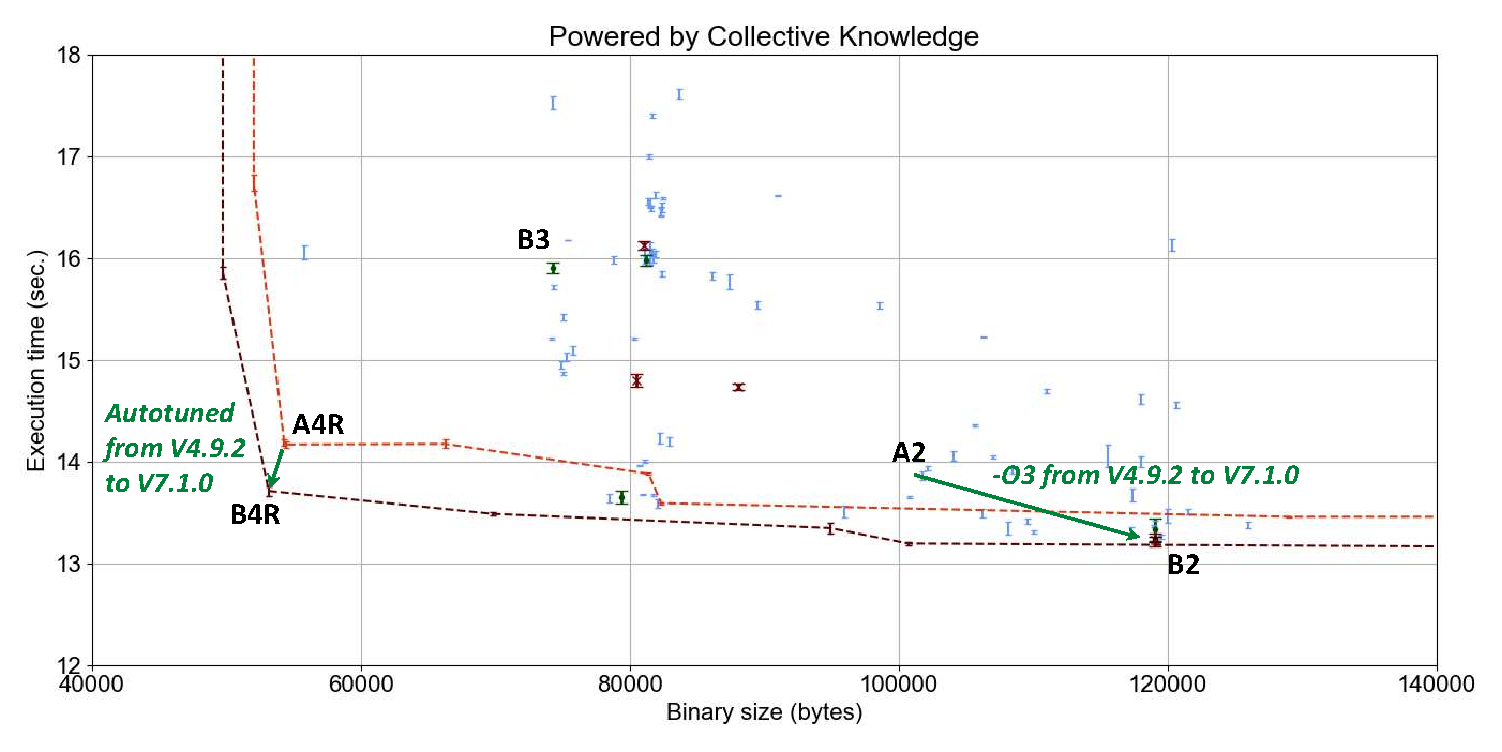
\includegraphics[width=5.2in]
      {ck-assets/2318dcb514171ad4-cropped.pdf} %CK_URL={2318dcb514171ad4-cropped.pdf}
      \vspace{0.1in}
          \begin{tabular}{|l|l|l|l|p{3.2in}|}
     \hline
      \textbf{ID} & \textbf{Compiler} & \textbf{Time (sec.)} & \textbf{Size (bytes)} & \textbf{Flags} \\ 
     \hline
      \textbf{ A2 } &  GCC 4.9.2  &  14.0 $\pm$ 0.1  &  101448  & {\small -O3 }\\
     \hline
      \textbf{ A4R } &  GCC 4.9.2  &  14.2 $\pm$ 0.1  &  54284  & {\small -O2 -flto }\\
     \hline
      \textbf{ B1 } &  GCC 7.1.0  &  38.8 $\pm$ 0.0  &  128376  & {\small  }\\
     \hline
      \textbf{ B2 } &  GCC 7.1.0  &  13.2 $\pm$ 0.1  &  119084  & {\small -O3 }\\
     \hline
      \textbf{ B3 } &  GCC 7.1.0  &  15.9 $\pm$ 0.1  &  74280  & {\small -Os }\\
     \hline
      \textbf{ B4R } &  GCC 7.1.0  &  13.7 $\pm$ 0.0  &  52424  & {\small -O2 -fgcse-after-reload -flto -fschedule-fusion -fno-ssa-phiopt -fno-tree-fre }\\
     \hline
    \end{tabular}     %CK_HTML={ck-assets/2318dcb514171ad4-table1.html}
      \vspace{0.1in}
     %CK_INTERACTIVE_GRAPH_PASSIVE={"cid":"2d41f89bcf32d4d4:df35fbf4dc6b3851", "where":"div#ck_interactive_54f71b367b787a13", "html":"rpi3-autotuning-zlib-encode-gcc7-interactive.html", "style":"rpi3-autotuning-zlib-encode-gcc7-interactive.style", "add_div":"yes", "add_box":"yes", "box_width":700, "remove_script_src":"yes"}
     \caption{
       Results of GCC 7.1.0 random compiler flag autotuning of zlib encode on RPi3 device 
       with a highlighted frontier (trading-off execution time and code size), 
       best combinations of flags on this frontier, and comparison with the results from GCC 4.9.2.
     }
     \label{fig:autotuning-zlib-encode-gcc7}
   \end{figure*}
   %\url{http://cknowledge.org/repo/web.php?wcid=graph:df35fbf4dc6b3851&subgraph=rpi3-autotuning-zlib-encode-gcc7-interactive}

   % === zlib encode GCC 7.1.0 reactions ==================================================================
   %CK={"action":"prepare_for_latex", "cid":"slide:e78a984c508cca1f", "file":"bae9e4979bd3bc4b-cropped.pdf", "path":"ck-assets", "ck_image":"yes", "ck_image_width":900}
   %CK={"action":"prepare_for_latex", "cid":"slide:e78a984c508cca1f", "file":"bae9e4979bd3bc4b-table1.tex", "uid":"59fa3e04026f23c5", "path":"ck-assets"}
   %CK={"action":"prepare_for_latex", "cid":"slide:e78a984c508cca1f", "file":"bae9e4979bd3bc4b-table1.html", "uid":"59fa3e04026f23c5", "path":"ck-assets"}
   \begin{figure*}[!htbp]
     \centering
      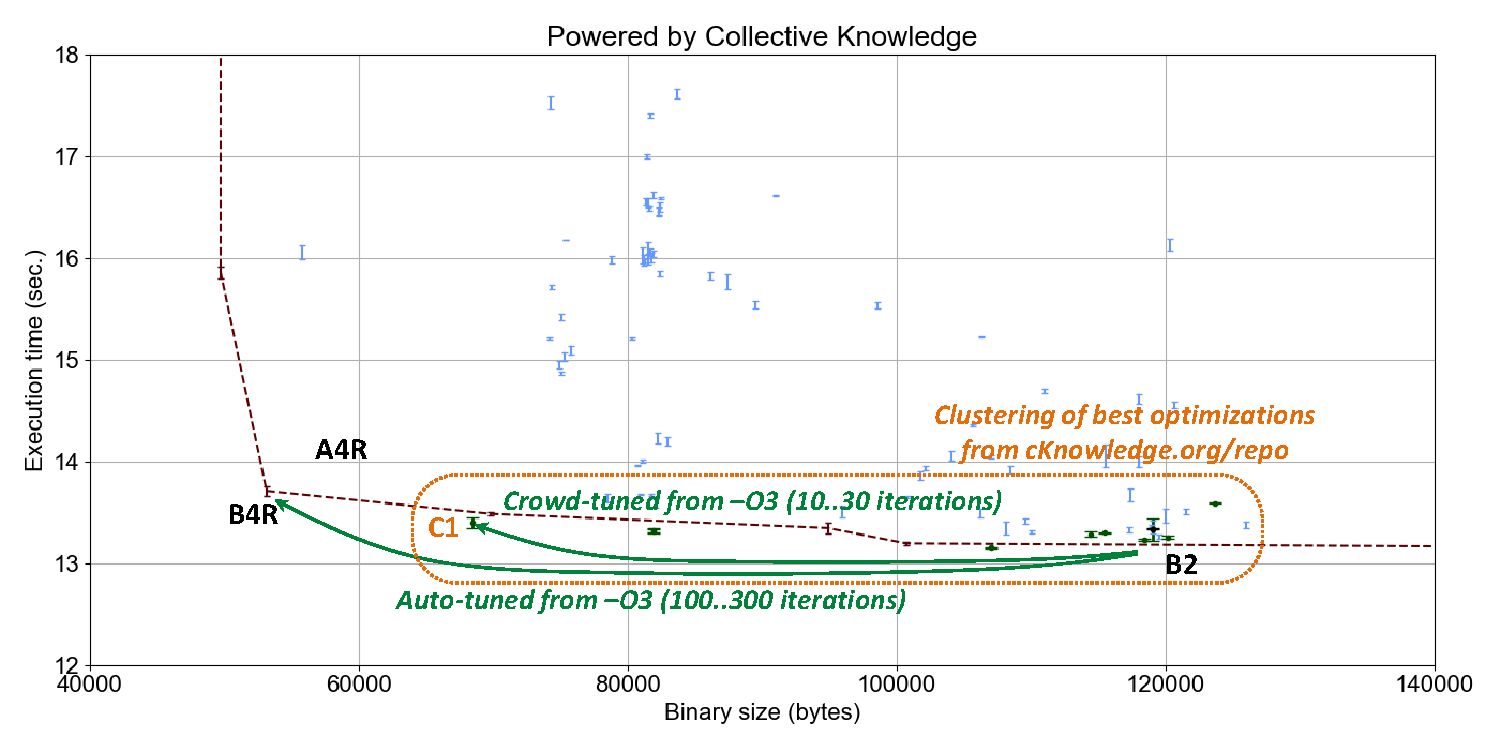
\includegraphics[width=5.8in]
      {ck-assets/bae9e4979bd3bc4b-cropped.pdf} %CK_URL={bae9e4979bd3bc4b-cropped.pdf}
      \vspace{0.1in}
          \begin{tabular}{|l|l|l|l|p{3.2in}|}
     \hline
      \textbf{ID} & \textbf{Compiler} & \textbf{Time (sec.)} & \textbf{Size (bytes)} & \textbf{Flags} \\ 
     \hline
      \textbf{ \href{http://cknowledge.org/repo/web.php?wcid=experiment:85a9d07941d187e4\&subpoint=c59cc63440c795a7}{A4R} } &  GCC 4.9.2  &  14.2 $\pm$ 0.1  &  54284  & {\small -O2 -flto }\\
     \hline
      \textbf{ \href{http://cknowledge.org/repo/web.php?wcid=experiment:50948cede943469a\&subpoint=381aef856bc24d3d}{B2} } &  GCC 7.1.0  &  13.2 $\pm$ 0.1  &  119084  & {\small -O3 }\\
     \hline
      \textbf{ \href{http://cknowledge.org/repo/web.php?wcid=experiment:3a9a0b4e4740a607\&subpoint=a8e09e075b5b4a38}{B4R} } &  GCC 7.1.0  &  13.7 $\pm$ 0.0  &  52424  & {\small -O2 -fgcse-after-reload -flto -fschedule-fusion -fno-ssa-phiopt -fno-tree-fre }\\
     \hline
      \textbf{ \href{http://cknowledge.org/repo/web.php?wcid=experiment:047ddbe5ef0ab588\&subpoint=0b17daf9418aaa6d}{C1} } &  GCC 4.9.2  &  13.3 $\pm$ 0.1  &  68464  & {\small -O3 -fno-inline -flto }\\
     \hline
    \end{tabular}     %CK_HTML={ck-assets/bae9e4979bd3bc4b-table1.html}
      \vspace{0.1in}
     \caption{
      Analyzing reactions of zlib encode to top most efficient GCC 7.1.0 optimizations shared by the community for RPi3 devices vs GCC 4.9.2.
     }
     \label{fig:autotuning-zlib-encode-gcc7-reactions}
   \end{figure*}
   %\url{http://cknowledge.org/repo/web.php?wcid=graph:47bfb7c243e4e907&subgraph=rpi3-autotuning-zlib-encode-gcc7-reactions-interactive}

Besides \textit{zlib}, we applied crowd-tuning with best found and shared optimizations 
to other RPi programs using \textit{GCC 4.9.2} and \textit{GCC 7.1.0}.
%
Table~\ref{fig:crowdtuning-all-rpi3-progs} shows reactions of these optimizations
with best trade-offs for execution time and code size.
%
One may notice that though \textit{GCC 7.1.0 -O3} level improves execution time
of most of the programs apart from a few exceptions, it also considerably degrades
code size in comparison \textit{GCC 4.9.2 -O3} level.
%
These results also confirm that neither \textit{-O3} nor \textit{-Os} on both 
\textit{GCC 4.9.2} and \textit{GCC 7.1.0} achieves best trade-offs for execution
time and code size thus motivating again our collaborative and continuous optimization
approach.

  % === all RPi3 results ==================================================================
  %CK={"action":"prepare_for_latex", "cid":"slide:2e8011124cb0c24d", "file":"1ea731443e29f6ce-table.tex", "uid":"4e08b1825a29cc6c", "path":"ck-assets"}
  %CK={"action":"prepare_for_latex", "cid":"slide:2e8011124cb0c24d", "file":"1ea731443e29f6ce-table.html", "uid":"4e08b1825a29cc6c", "path":"ck-assets"}
  \begin{table*}[]
    \centering
         \begin{tabular}{|l|l|p{0.9in}|p{0.9in}|p{3.0in}|}
     \hline
      \textbf{Workload} & \textbf{Compiler} & \textbf{Time improvement over -O3 (-O3 time in brackets)} & \textbf{Binary size improvement over -O3 (-O3 size in brackets)} & \textbf{Flags} \\ 
     \hline
      \textbf{ 7z encode } &  GCC 4.9.2  &  ~ 1.02 (5.5 $\pm$ 0.1)  &  ~ 1.52 (859728)  & {\small -O3 -fno-inline -flto }\\
     \hline
      \textbf{ 7z encode } &  GCC 7.1.0  &  no (6.0 $\pm$ 1.0)  &  no (887464)  & {\small -O3 }\\
     \hline
      \textbf{ ccrypt encrypt } &  GCC 4.9.2  &  no (7.0 $\pm$ 2.0)  &  no (61772)  & {\small -O3 }\\
     \hline
      \textbf{ ccrypt encrypt } &  GCC 7.1.0  &  ~ 1.16 (7.6 $\pm$ 0.1)  &  ~ 1.00 (59996)  & {\small -O3 -fno-auto-inc-dec -fguess-branch-probability -fipa-pure-const -freorder-blocks -fselective-scheduling2 -ftree-ccp -fno-tree-pre -ftree-tail-merge }\\
     \hline
      \textbf{ ccrypt encrypt } &  GCC 7.1.0  &  ~ 1.06 (7.6 $\pm$ 0.1)  &  ~ 1.04 (59996)  & {\small -O3 -fdelete-null-pointer-checks -fno-indirect-inlining -fipa-cp-alignment -fno-ipa-pure-const -freciprocal-math -fsched-spec-insn-heuristic -fschedule-insns2 -fno-ssa-phiopt -fno-tree-ch -ftree-copy-prop -fno-tree-sink -fno-tree-switch-conversion -funsafe-loop-optimizations -funsafe-math-optimizations }\\
     \hline
      \textbf{ gzip decode } &  GCC 4.9.2  &  ~ 1.04 (4.2 $\pm$ 0.0)  &  ~ 1.12 (85956)  & {\small -O3 -fno-inline -flto }\\
     \hline
      \textbf{ gzip decode } &  GCC 7.1.0  &  ~ 1.04 (4.2 $\pm$ 0.0)  &  ~ 1.18 (90568)  & {\small -O3 -fno-inline -flto }\\
     \hline
      \textbf{ gzip decode } &  GCC 7.1.0  &  ~ 1.08 (4.2 $\pm$ 0.0)  &  ~ 0.81 (90568)  & {\small -O3 -fno-cprop-registers -flto -funroll-all-loops }\\
     \hline
      \textbf{ gzip encode } &  GCC 4.9.2  &  ~ 0.98 (12.3 $\pm$ 0.1)  &  ~ 1.10 (85956)  & {\small -O3 -fno-omit-frame-pointer -fno-tree-loop-optimize }\\
     \hline
      \textbf{ gzip encode } &  GCC 7.1.0  &  ~ 1.01 (12.3 $\pm$ 0.8)  &  ~ 1.18 (90568)  & {\small -O3 -fno-inline -flto }\\
     \hline
      \textbf{ minigzip decode } &  GCC 4.9.2  &  ~ 1.24 (10.0 $\pm$ 4.0)  &  ~ 1.60 (101432)  & {\small -O3 -fno-inline -flto }\\
     \hline
      \textbf{ minigzip decode } &  GCC 4.9.2  &  ~ 1.32 (10.0 $\pm$ 4.0)  &  ~ 1.00 (101432)  & {\small -O3 -fselective-scheduling2 -fno-tree-pre }\\
     \hline
      \textbf{ minigzip decode } &  GCC 7.1.0  &  ~ 1.14 (8.0 $\pm$ 3.0)  &  ~ 1.76 (119088)  & {\small -O3 -fno-inline -flto }\\
     \hline
      \textbf{ minigzip encode } &  GCC 4.9.2  &  ~ 0.89 (9.9 $\pm$ 0.0)  &  ~ 1.60 (101432)  & {\small -O3 -fno-inline -flto }\\
     \hline
      \textbf{ minigzip encode } &  GCC 7.1.0  &  ~ 1.00 (9.6 $\pm$ 0.0)  &  ~ 1.76 (119088)  & {\small -O3 -fno-inline -flto }\\
     \hline
      \textbf{ rhash sha3 } &  GCC 4.9.2  &  ~ 1.00 (4.8 $\pm$ 0.0)  &  ~ 1.12 (14848)  & {\small -O3 -flto }\\
     \hline
      \textbf{ rhash sha3 } &  GCC 7.1.0  &  ~ 1.35 (5.2 $\pm$ 0.0)  &  ~ 1.30 (16396)  & {\small -O3 -fno-inline -flto }\\
     \hline
      \textbf{ rhash sha3 } &  GCC 7.1.0  &  ~ 1.48 (5.2 $\pm$ 0.0)  &  ~ 1.07 (16396)  & {\small -O3 -fno-schedule-insns -ftracer }\\
     \hline
      \textbf{ sha512sum sha512 } &  GCC 4.9.2  &  ~ 1.12 (7.8 $\pm$ 0.0)  &  ~ 1.06 (125372)  & {\small -O3 -fno-schedule-insns -fselective-scheduling2 }\\
     \hline
      \textbf{ sha512sum sha512 } &  GCC 7.1.0  &  ~ 1.22 (7.3 $\pm$ 0.0)  &  ~ 1.07 (121180)  & {\small -O3 -fno-predictive-commoning -fno-schedule-insns -funroll-loops }\\
     \hline
      \textbf{ unrar } &  GCC 4.9.2  &  ~ 0.97 (18.0 $\pm$ 4.0)  &  ~ 1.38 (326572)  & {\small -O3 -fno-inline -flto }\\
     \hline
      \textbf{ unrar } &  GCC 4.9.2  &  ~ 1.13 (18.0 $\pm$ 4.0)  &  ~ 0.80 (326572)  & {\small -O3 -fno-section-anchors -fselective-scheduling2 -fno-tree-forwprop -funroll-all-loops }\\
     \hline
      \textbf{ unrar } &  GCC 7.1.0  &  ~ 0.96 (18.0 $\pm$ 6.0)  &  ~ 1.38 (326572)  & {\small -O3 -fno-inline -flto }\\
     \hline
      \textbf{ unrar } &  GCC 7.1.0  &  ~ 1.07 (18.0 $\pm$ 6.0)  &  ~ 0.78 (326572)  & {\small -O3 -fno-tree-ter -funroll-all-loops }\\
     \hline
    \end{tabular}     %CK_HTML={ck-assets/1ea731443e29f6ce-table.html}
    \caption{
      Best found improvements (degradations) in execution time and binary size 
      for several important RPi3 programs 
      as reactions to top most efficient shared optimizations 
      for GCC 4.9.2 and GCC 7.1.0.
    }
    \label{fig:crowdtuning-all-rpi3-progs}
  \end{table*}

Indeed, a dozen of shared most efficient optimizations at \href{http://cKnowledge.org/repo}{cKnowledge.org/repo} 
is enough to either improve execution time of above programs by up to 1.5x or code size by up to 1.8x or even
improve both size and speed at the same time.
%
It also helps end-users find best optimization no matter which compiler, environment and hardware are used.

We can also notice that 11 workloads (computational species) 
share \textit{-O3 -fno-inline -flto} combination of flags 
to achieve best trade-off between execution time and code size.
%
This result supports our original research to use workload features, 
hardware properties, crowd-tuning and  machine learning
to predict such optimizations~\cite{Fur2009,29db2248aba45e59:a31e374796869125,cm:29db2248aba45e59:cd11e3a188574d80}.
%
However, in contrast with past work, we are now able
to gradually collect a large, realistic (i.e. not randomly
synthesized) set of diverse workloads with the help of the
community to make machine learning statistically meaningful.

All scripts to reproduce experiments from this section are available in the following CK entries:

\begin{flushleft}
\texttt{\$ ck find script:rpi3-zlib-decode*\newline
\$ ck find script:rpi3-zlib-encode*\newline
\$ ck find script:rpi3-all-autotune}
\end{flushleft}
